\subsection{Desenvolver Suíte de Testes Automatizados}

A suíte de testes automatizados será responsável em garantir o correto funcionamento da integração entre os sistemas envolvidos, ou seja prover um meio onde possa ser testado tanto o Webservice do GSAN quanto a Interface Agi implementada para o Asterisk, para essa situação foram utilizados recursos do JUnit para criação dos cenários, execução dos testes e identificação de falhas, quanto recursos do framework Asterisk-Java para simular e controlar uma chamada telefônica com parâmetros dinâmicos.   

Cada classe de teste deve implementar uma interface do framework Asterisk-Java chamada \textit{PropertyChangeListener} e posteriormente ser registrada como \textit{Listener} em uma classe da suíte chamada \textit{SuiteAsteriskListener}, que atua como uma escuta de modificações ocorridas em  canais, tais canais que representam as chamadas existentes na ferramenta. 
A suíte de testes está configurada para sempre antes de executar um teste realiza primeiro o Login na ferramenta Asterisk e ao final da execução do teste efetuar o Logoff, somente após o login é possível iniciar a simulação das chamadas para os contextos de testes, abaixo está demonstrado o funcionamento na forma de diagrama de sequência conforme a figura \ref{figura:diagramaSeq2Via} abaixo;

\begin{figure}[!htb]
	\centering
	\caption{Diagrama de sequência utilizando a suíte de teste.}
	\label{figura:diagramaSeq2Via}
	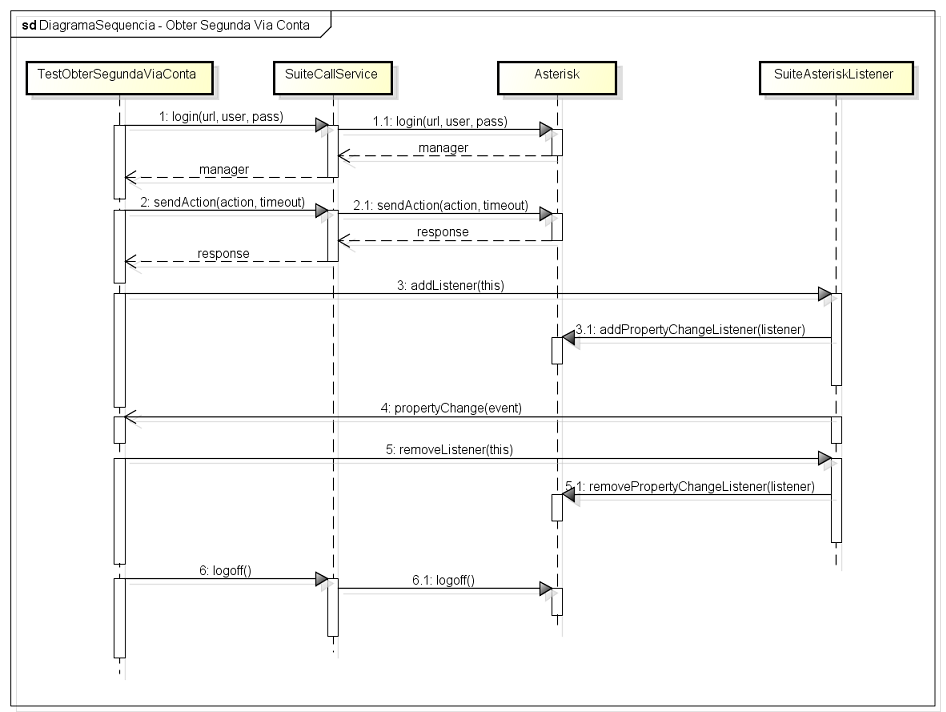
\includegraphics{figuras/diagramaSequenciaObter2ViaTest.png}
	\legend {\fontsize{10}{12}\selectfont {Fonte: Autoria Própria}.}
\end{figure}

% Figura para demonstrar a classe de teste - classe_teste_suite.png
% Para execução dos testes foi necessário realizar algumas customizações na ferramenta Asterisk, 
% desabilitar o iptables, 
% contexto de teste,
% Criação/Habilitar o user manager para remote conection.
% /etc/asterisk/manager.conf
% [general]
% enabled=yes 
% port=5038
% bindaddr=0.0.0.0
% displayconnects=yes
% permit=0.0.0.0/0.0.0.0

% [manager]
% secret=pa55w0rd 
% allow=0.0.0.0/0.0.0.0
% read=system,call,log,verbose,command,agent,user
% write=system,call,log,verbose,command,agent,user
% permit=0.0.0.0/0.0.0.0

